\documentclass{beamer}

\usepackage{graphicx}
\usepackage{tikz}

% this actually isn't totally hideous:
\usetheme[numbering=counter, progressbar=foot, sectionpage=none]{metropolis}

\graphicspath{{../figures/}}

\title{Composable Concurrency Models}
\date{November 19, 2016}
\author{Dan Stelljes}

\begin{document}
  \maketitle

  \section{Introduction}
  
  \begin{frame}
    \begin{figure}
      \begin{tikzpicture}
        \onslide<1->{
          \node at (0,0) {
            
\includegraphics[width=300pt]{browser}
          };
        }

        \onslide<2>{
          \path (-2.25,2.75) [draw=none, fill=darkgray, opacity=0.75] ellipse (60pt and 25pt);
          \node [text=white] at (-2.25,2.75) {
            Multiple tabs
          };

          \draw (2.25,2.25) [draw=none, fill=darkgray, opacity=0.75] ellipse (60pt and 25pt);
          \node [text=white] at (2.25,2.25) {
            Suggestions
          };

          \draw (0,0.5) [draw=none, fill=darkgray, opacity=0.75] ellipse (60pt and 25pt);
          \node [text=white] at (0,0.5) {
            Page rendering
          };

          \draw (-3,-1.5) [draw=none, fill=darkgray, opacity=0.75] ellipse (60pt and 25pt);
          \node [text=white] at (-3,-1.5) {
            Event handling
          };

          \draw (2.5,-1.5) [draw=none, fill=darkgray, opacity=0.75] ellipse (60pt and 25pt);
          \node [text=white] at (2.5,-1.5) {
            Background processes
          }; 
        }

        \onslide<3>{
          \node at (0,-0.62) {
            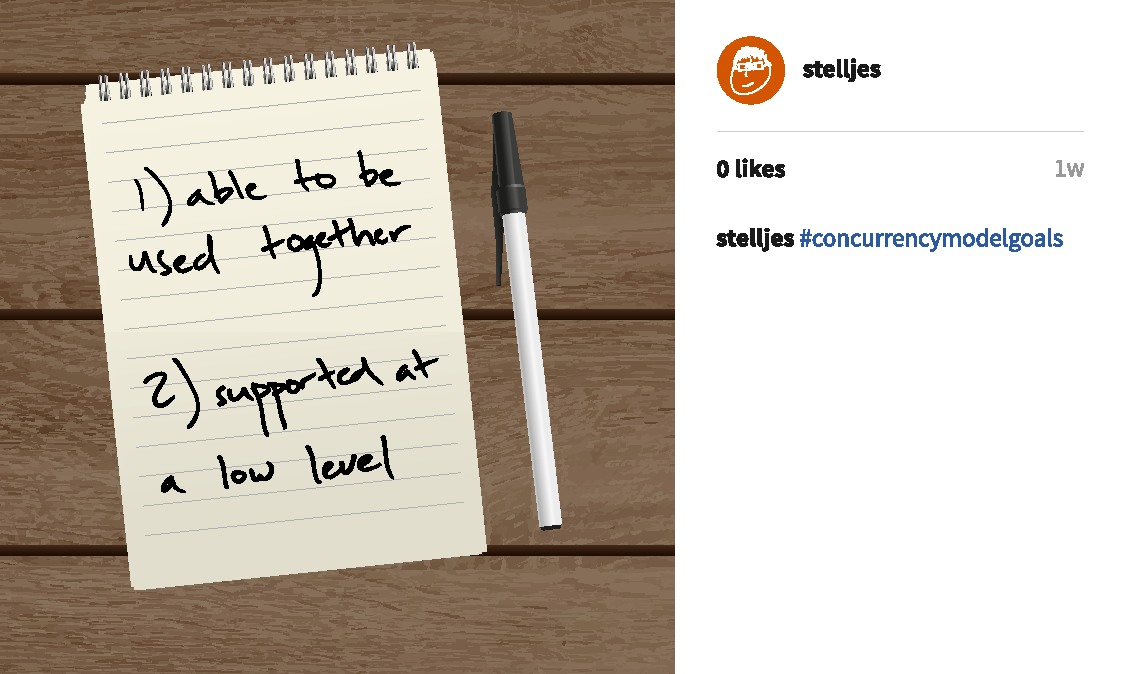
\includegraphics[width=220pt]{goals}
          };
        }
      \end{tikzpicture}
    \end{figure}
  \end{frame}
\end{document}
